\section{Resultats}

Dans cette partie, nous verrons les résultats et déductions qui ont été faites à partir des différentes approches. Elle évoquera aussi ce qui à été accompli et ce qui reste à faire.

Les résultats et déductions seront cités par ordre chronologique, il est donc normal que certaines approches soient invalidés.

L'implémentation et le fonctionnement interne des application sont explicités dans le manuel technique, malgré tout, certaines implémentations seront expliquées ici pour justifier les décisions prises durant le stage.

De plus, grâce au développement en parallèle d'un solveur en programmation par contraintes \autocite{choco} par Mr Bourreau nous apporte un certain recul sur les données reçus.

	\subsection{Bruteforce}
	
	Les résultats de la bruteforce suivent ce qui avait été prédit. Malgré un certain niveau d'optimisation du programme, la plus grande instance résolue est de taille 6.
	
	Le puzzle de taille 7 n'as pas pu être parcouru en 9 heures de calcul. Malgré tout, la première solution de l'instance se trouvait au n\oe ud 10548049 et à été trouvée en 31.7344 secondes en rowscan.
	
	D'après les résultats le choix de variable le plus performant est le \enquote{rowscan} [\autoref{annexe:bruteforce}]. On remarque aussi que le nombre de n\oe uds total et le temps écoulé augmente de façon exponentielle en fonction de la taille de l'instance.
	
	\begin{note}
		La programmation par contrainte à l'air d'être plus performante que le parcours naïf en bruteforce d'après la \autoref{fig:results_bruteforce_graphique_compare}.
	\end{note}
	
	\subsection{Smartforce}
	
	Les valeurs étalons pour les choix de variables dynamiques (optimiste/pessimiste) qui ont été implémentés sur un modèle \textbf{CaPi}, elles se sont avérées moins performantes qu'un parcours basique.
	
	La raison est simple : il est possible de recréer le même cas en parcourant de différentes façons. Par conséquent, le nombre de n\oe uds augmente sans pour autant parcourir de nouvelles possibilités.
	
	\begin{exmp}
		Soit un plateau composé de deux cases et par conséquent, de deux pièces. Si je pose d'abord ma pièce sur la première case, puis sur la deuxième. Le résultat sera le même que si je pose d'abord l'autre pièce sur la deuxième case puis que je fasse la première.
		
		Donc, j'ai deux façons de trouver le même résultat.
	\end{exmp}
	
	Le choix de valeur dynamique, décident du chemin à chaque n\oe uds, il fait plusieurs fois la même combinaison, mais avec un chemin différent.
	
	Les tests effectués sur les choix de valeur dynamiques ont obtenus les mêmes résultats que pour le \textbf{rowscan} car aucune mise à jour par propagation n'a pas été implémentée pour CaPi (non performant).
	
	Le modèle \textbf{BoCo} est en cours d'implémentation, mais ne fournit pas des résultats pertinent. Le problème se trouve dans le mécanisme de mise à jour par propagation.
	
	\subsection{Corolles}
	
	Afin de pouvoir assimiler le fonctionnement des corolles dans la pratique, il est important de tenir compte de la quantité volumineuse d'information que génère ce modèle (voir \autoref{annexe:smartforce}).
	
	A titre d'exemple, le nombre de corolles en hamming 2 pour une instance de taille 6 (non rotationnées) est de 850694772. Avec un stockage non optimisé des corolles, l'espace occupé par ces corolles s'élève à environ 90GB.
	Par extension, on peux en déduire que pour une instance de taille 7, l'espace occupé par l'ensemble des corolles avoisinera au moins 1TB (en prenant la valeur de la \autoref{table:count_hamming_2} comme valeur max, et en supposant que l'espace occupé par une corolle est la même).
	
	Ce stockage avait un défaut important, il n'était pas optimisé pour le stockage mais pour pouvoir manipuler avec aise les corolles.
	
	Une corolle etait stockée de cette manière : chaque pièce était identifiée par un numéro et sa rotation, l'ensemble des pièces était séparés par un charactère (;) et disposés dans un ordre spécifique (voir \autoref{fig:corolle}). Suivait ensuite la frontière, composée de couleurs qui étaient aussi séparés par un charactère (;). Évidemment, si la corolle etait réduite, les cases et frontières manquantes étaient remplacées par un vide.
	\begin{exmp}
		\lstinline[columns=fixed]{0:0;5:1;6:0;;|3;4;5;6;7;;;;;;;0}
	\end{exmp}
	
	Une corolle étant une sous-partie du plateau, un ensemble de corolles peux être représenté sous forme d'arbre. Lors de la création de la corolle, on parcours tout simplement l'arbre en profondeur. Ainsi, dans le fichier, deux lignes adjacentes se ressemblent fortement.
		\begin{figure}[H]
			\centering
			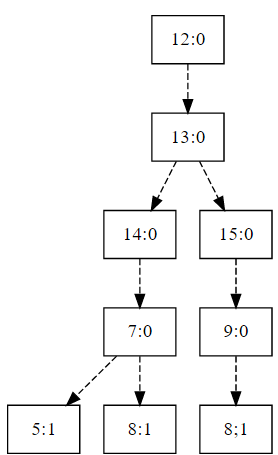
\includegraphics[width=0.3\linewidth]{images/corolle_tree}
			\caption{Représentation sous forme d'arbre d'un exemple de corolles possibles}
			\label{fig:corolle_tree}
		\end{figure}
	
	
	\begin{exmp}\ 
		
		\begin{lstlisting}
0:0;5:1;6:0;;|3;4;5;6;0;;;;;;;0
0:0;5:1;7:0;;|3;4;5;3;0;;;;;;;0
		\end{lstlisting}
		
	\end{exmp}
	
	On peux donc optimiser en spécifiant à partir quelle pièce se fait l'optimisation.
	
	Nous obtenons donc :
	
	\begin{exmp}
		\ 
		
		\begin{lstlisting}
0>0:0;5:1;6:0;;|3;4;5;6;0;;;;;;;0
1>7:0;;|3;4;5;3;0;;;;;;;0
		\end{lstlisting}
	\end{exmp}
	
	Grâce à ce procédé, le fichier de 90GB est passé à 20GB, ce qui nous donne une optimisation de $70\%$ environ. Ceci étant, il est intéressant de noter que la compression de ces fichier grâce à LZMA \autocite{wiki:lzma} permet de réduire de $98\%$ le volume du fichier. Mais la compression exige un certain délai afin de pouvoir exploiter les fichiers compréssés, ce qui limite son utilisation.
	
	Il existe une dernière approche, qui se base sur un constant simple :
	dans une corolle de hamming 1, les pièces adjacentes à la pièce centrale sont indépendantes les uns des autres. Il suffit donc de lister à chaque position les pièces qui peuvent y être posés, puis lorsqu'il y a nécessité de créer une corolle, parcourir les positions en fixant une pièce. Toutes les corolles sont possibles, tant que le chemin ne possède pas deux fois la même pièce.
	
	\begin{exmp}
		Reprenons l'exemple précédent en y rajoutant une ligne:
		
		nous avons donc
		\begin{tabular}{|c|c c c|}
			\hline 
			Positions & 0 & 1 & 2 \\ 
			\hline 
			 & $0:0$ & $5:1$ & $6:0$ \\
			  & $0:0$ & $5:1$ & $7:0$ \\
 & $0:0$ & $6:1$& $7:0$ \\
 \hline
		\end{tabular}
		
		il suffit donc d'enregistrer dans le fichier :
		
		\begin{lstlisting}
			0:0;5:1;6:0
			   ;6:1;7:0
		\end{lstlisting}
		
		Tant que l'on ne prend pas \lstinline[columns=fixed]{0:0;6:1;6:0} tous les autres cas sont possibles.
	\end{exmp}
	
	Plus théoriquement, on fait un produit cartésien entre les ensembles de chaque position et l'on en obtient une corolle.
	
	Le soucis, c'est que cette méthode fonctionne en hamming 1 car les pièces de H1 sont indépendantes de les unes des autres. En H2, l'approche est plus complexe : les pièces de H2 sont dépendants des pièces de H1. Or, on vient de déterminer un moyen de stocker les corolles. Il suffit de spécifier quel chemin emprunter en H1 (l'identifier) puis d'appliquer la même méthode des ensembles, mais pour les pièces de H2.
	
	Ainsi, on peux obtenir, en minimisant la taille des fichiers, toutes les corolles possibles.
	
	Malheureusement cette dernière approche n'as pas pu être mise en place faute de temps.
	
	\newpage
	
	\subsection{Liens dansants~\autocite{knuth2000dancing}}
	Le principe des liens dansants est à la fois complexe au niveau théorique que pratique. L'intérêt de cette approche est de réduire la quantité de données à consulter lors du parcours de l'arbre sans pour autant supprimer ou libérer ces données (pour pouvoir les réutiliser plus tard). Son principe est simple, il repose sur une base de liste doublement chainée : un élément est relié à l'élément suivant et précédent. Tous les éléments sont aussi répertoriés dans un tableau. Lorsque l'on souhaite masquer un élément du parcours, il suffit de chainer l'élément qui le précède à celui qui le suit (et vice-versa). De cette façon, l'élément actuel est ignoré car il n'est plus dans la chaine, mais, il est toujours répertorié. Lorsque l'on souhaite le remettre dans la chaine, il suffit de lire quel est l'élément qui le suit, puis de chainer cet élément à soi-même (pareil pour l'élément qui le précède ; il faut se chainer comme l'élément qui le suit).
	
	\begin{defn}
		Soit $S[x]$ et $P[x]$ pointant respectivement vers le successeur et le prédécesseur d'un élément. L'opération ci-dessous supprime un l'élément :
		
		\[
			L[R[x]] \leftarrow L[x], R[L[x]] \leftarrow R[x]
		\]
		
		Et à l'inverse, cette opération le rétablit :
		
		\[
			L[R[x]] \leftarrow x, R[L[x]] \leftarrow x
		\]
	\end{defn}
	
	Son emploi est très bénéfique dans des application de parcours d'arbre. Mais son implémentation peux être faite à plusieurs niveaux : la liaison des domaines dans les différents modèles (CaPi et BoCo) mais surtout dans le modèle des corolles.
	
	On chaine une corolle $C$ avec la corolle qui la précède et qui la suit (principe des liens dansants). On fait la même chose avec les pièces qui composent C : on chaine la pièce avec la position suivante et précédente de la corolle (on \enquote{met} $C$ sous forme de liens dansants). Ensuite, on chaine chaque pièce avec la prochaine (et précédente) occurrence de cette pièce (à la même position) dans la liste des corolles. Au final on obtient une liste 6-tuplement chainée.
	
	Grâce à cette quantité de liaison, lors de la pose d'une corolle, on peux rapidement l'enlever du parcours, on peux aussi dénier toutes les corolles qui ont des occurrences des pièces déjà posées. Toutes ces mises à jour sont fait en $k$ étapes, $k$ représentant le nombre de corolles à dénier.

	\subsection{GPU}
	
	Une fois le système de corolles et de liens dansants mis en place, le but était d'utiliser les capacités d'un GPU (carte graphique) afin de paralléliser les calculs. En effet, le GPU se distingue par sa quantité astronomique de c\oe urs, ce qui le rends imbattable sur les problèmes où les calculs peuvent être parallélisés.